\documentclass[t, utf8, 10pt]{beamer}
\usepackage[ngerman]{babel}
\usepackage{bera}
\usepackage{fontawesome}
\usepackage{pifont}
\usepackage{color}
\usepackage{listings}
\usepackage{url}

\setbeamertemplate{navigation symbols}{}

\lstdefinestyle{customc}{
  belowcaptionskip=1\baselineskip,
  breaklines=true,
  frame=single,
  xleftmargin=\parindent,
  language=C,
  showstringspaces=false,
  basicstyle=\scriptsize\ttfamily,
  keywordstyle=\bfseries\color{green!40!black},
  commentstyle=\itshape\color{purple!40!black},
  identifierstyle=\color{blue},
  stringstyle=\color{orange},
}

\lstdefinestyle{customfortran}{
  belowcaptionskip=1\baselineskip,
  breaklines=true,
  frame=single,
  xleftmargin=\parindent,
  language=Fortran,
  showstringspaces=false,
  basicstyle=\scriptsize\ttfamily,
  keywordstyle=\bfseries\color{green!40!black},
  commentstyle=\itshape\color{purple!40!black},
  identifierstyle=\color{blue},
  stringstyle=\color{orange},
}

\lstdefinestyle{custompython}{
  belowcaptionskip=1\baselineskip,
  breaklines=true,
  frame=single,
  xleftmargin=\parindent,
  language=Python,
  showstringspaces=false,
  basicstyle=\scriptsize\ttfamily,
  keywordstyle=\bfseries\color{green!40!black},
  commentstyle=\itshape\color{purple!40!black},
  identifierstyle=\color{blue},
  stringstyle=\color{orange},
}

\hypersetup{%
  pdftitle={Python im Unterricht}
  ,pdfauthor={Gert-Ludwig Ingold <gert.ingold@physik.uni-augsburg.de>}
  ,pdfsubject={Linux Infotag 2018, Augsburg, 21.4.2018}
  ,pdfkeywords={Python, teaching, jupyter, nbgrader}
}

\graphicspath{{./img/}}

\begin{document}

\begin{frame}
 \vspace{4truecm}
 \begin{center}
  \structure{\LARGE Python im Unterricht}\\[0.3truecm]
  {\large Gert-Ludwig Ingold}

  \vspace{2truecm}
  \faicon{github}
  \texttt{\normalsize git clone https://github.com/gertingold/lit2018.git}
 \end{center}
\end{frame}

\begin{frame}{Über mich}
 \begin{itemize}
  \item seit 1994 Theoretischer Physiker an der Universität Augsburg
  \item seit 2010 auch Vorlesungen zum Programmieren\\
	\url{gertingold.github.io}
  \item 2015--2017 Erasmus+-Projekt iCSE4school\quad
        \raisebox{-0.25truecm}{\includegraphics[width=0.27\textwidth]{eu_flag_co_funded_pos_[rgb]_right}}\\
	Anwendung von SageMath im gymnasialen Unterricht
        \begin{itemize}
	 \item Uniwersytet Śląski, Kattowitz
	 \item Simula Research Laboratory, Oslo
	 \item Universität Augsburg
	 \item Gymasien in Chorzów und Warschau
	 \item EDU-RES Chorzów
	\end{itemize}
  \item 2017--2019 Erasmus+-Projekt Jupyter@edu\quad
        \raisebox{-0.25truecm}{\includegraphics[width=0.27\textwidth]{eu_flag_co_funded_pos_[rgb]_right}}\\
	Anwendung von Jupyter Notebooks an Universitäten
        \begin{itemize}
	 \item Uniwersytet Śląski, Kattowitz
	 \item Universität Augsburg
         \item European University Cyprus, Nikosia
	 \item Universidade Portucalense, Porto
	 \item EDU-RES Chorzów
	\end{itemize}
 \end{itemize}
\end{frame}

\begin{frame}{Welche Programmiersprache?}

 \vspace{1truecm}
 \uncover<2>{\includegraphics[width=0.5\textwidth]{python-logo-master-v3-TM}}
 \begin{itemize}
  \item Eignet sich die Programmiersprache für Anfänger?
        \uncover<2>{\textcolor{green!70!black}{\ding{52}}}
  \item Eignet sich die Programmiersprache zur Verwendung
        in anderen Fächern, z.B. im naturwissenschaftlichen
        Unterricht?
        \uncover<2>{\textcolor{green!70!black}{\ding{52}}}
  \item Eignet sich die Programmiersprache auch für reale
        Anwendungen in Wissenschaft und Industrie?
        \uncover<2>{\textcolor{green!70!black}{\ding{52}}}
 \end{itemize}
\end{frame}

\begin{frame}{Was andere denken}
 \begin{columns}
  \begin{column}{0.58\textwidth}
   \includegraphics[width=\textwidth]{Top39-700_4}
  \end{column}
  \begin{column}{0.42\textwidth}
   \vspace{-2truecm}

   \fontsize{5}{6}\selectfont
   http://cacm.acm.org/blogs/blog-cacm/176450-python-is-now-the-most-popular-introductory-teaching-language-at-top-us-universities/fulltext
  \end{column}
 \end{columns}

 \vspace{\baselineskip}
 most popular languages on Github 2017 (\url{octoverse.github.com})

 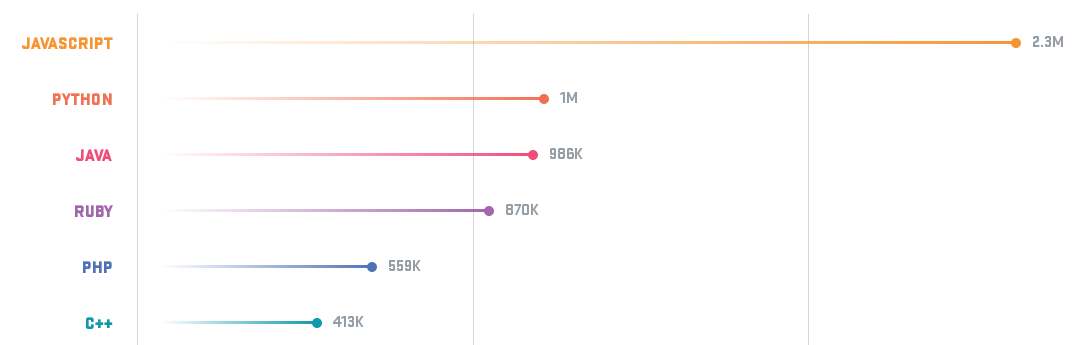
\includegraphics[width=\textwidth]{Screenshot-2018-4-12_GitHub_Octoverse_2017}
\end{frame}

\begin{frame}[fragile]{Warum Python?}
 \structure{niedrige Lernbarriere durch expressiven und gut lesbaren Code}

 \vspace{0.3truecm}
 \begin{columns}[t]
  \begin{column}{0.5\textwidth}
   Python
   \lstset{style=custompython}
   \begin{lstlisting}
   for n in range(5):
       print(n, n**2)
   \end{lstlisting}

   \begin{footnotesize}
    \begin{itemize}
     \setlength{\itemindent}{-10pt}
     \item Einrückungen sind syntaktisch relevant
     \item keine Typdeklaration (\textit{duck typing})
    \end{itemize}
   \end{footnotesize}
  \end{column}
  \begin{column}{0.5\textwidth}
   Fortran
   \lstset{style=customfortran}
   \begin{lstlisting}
     PROGRAM Squares
     DO n = 0, 4
        PRINT '(2I4)', n, n**2
     END DO
     END PROGRAM Squares
   \end{lstlisting}
  \end{column}
 \end{columns}
  
 \vspace{0.5truecm}
 \begin{columns}
  \begin{column}{0.7\textwidth}
   C
   \lstset{style=customc}
   \begin{lstlisting}
    #include <stdio.h>

    void main(){
       int n;
       for(n = 0; n < 5; n++){
             printf("%4i %4i\n", n, n*n);
       }
    }
   \end{lstlisting}
  \end{column}
  \begin{column}{0.3\textwidth}
   \strut
  \end{column}
 \end{columns}
\end{frame}

\begin{frame}{Warum Python?}
 \begin{itemize}
  \item frei verfügbar für Windows, MacOS, Linux, \ldots
  \item umfangreiche Distributionen frei verfügbar\\
        für wissenschaftliche Anwendungen, Datenanalyse z.B.\\
        Anaconda (\url{www.anaconda.com})
 \end{itemize}
\end{frame}

\begin{frame}{Warum Python?}
 \structure{interpretierte Sprache erlaubt explorierendes Lernen}
\end{frame}

\begin{frame}{Das wissenschaftliche Ökosystem von Python}
 \begin{columns}
  \begin{column}{0.44\textwidth}
   \raisebox{-0.63\textheight}{\includegraphics[width=\textwidth]{sln_logo}}

   \begin{footnotesize}
    \url{https://www.scipy-lectures.org/}
   \end{footnotesize}
  \end{column}%
  \begin{column}{0.56\textwidth}
   \begin{small}
    \begin{itemize}
     \setlength{\itemindent}{-10pt}
     \item Matrizen als Objekte (\texttt{ndarray})
     \item numerische Integration und Lösung von Differentialgleichungen
     \item lineare Algebra
     \item statistische Funktionen
     \item spezielle Funktionen
     \item graphische Darstellungen
     \item Bildbearbeitung
     \item maschinelles Lernen
     \item Bearbeitung großer Datensätze
     \item symbolische Mathematik
     \item und vieles mehr \ldots
    \end{itemize}
   \end{small}
  \end{column}
 \end{columns}
\end{frame}

\begin{frame}{Warum Python?}
 \begin{itemize}
  \item freie Verfügbarkeit für Windows, MacOS, Linux
  \item umfangreiche freie Programmbibliotheken, auch
        im wissenschaftlichen Bereich
  \item interpretierte Sprache
  \item keine Fixierung auf ein Programmierparadigma\\
        objektorientiertes Programmieren möglich\\
        Elemente der funktionalen Programmierung
 \end{itemize}
\end{frame}

\begin{frame}{Jupyter notebook}
\end{frame}

\end{document}
